% ================== Preamble ===================================================

\documentclass[11pt, a4paper, portrait]{scrreprt}
\input{LaTeX-Files/Preamble.tex}
\begin{document}

% ================== Deckblatt ==================================================

\pagenumbering{gobble}
% ================== Frontseite ==================================================
\thispagestyle{empty}
\begin{center}

\vspace*{3cm}

{\Huge\bfseries HSLU Mobile Apps - Android Jetpack Compose - AI First\par}

\vspace{2cm}

{\Large Wirtschaftsprojekt Herbstsemester 2025\par}

\vspace{3cm}

{\Large\textbf{Autoren:} Raphael Eiholzer und Samuel Kurmann\par}

{\Large\textbf{Betreuer:} Jürg Nietlispach\par}

\vfill

{\large Hochschule Luzern – Departement Informatik\par}
{\large Rotkreuz, Schweiz\par}
{\large \today\par}

\end{center}

\newpage
\newpage

\noindent
\fontsize{12}{14}
\textbf{Wirtschaftsprojekt an der Hochschule Luzern -- Informatik} \\ \vspace*{0.6cm}

{\fontsize{11}{12}\selectfont
\noindent
\textbf{Titel: HSLU Mobile Apps - Android Jetpack Compose - AI First} \\ \vspace*{0.2cm}

\noindent
\textbf{Student: Samuel Kurmann} \newline \newline
\textbf{Student: Raphael Eiholzer} \newline \newline
\textbf{Studiengang:} BSc Informatik \newline \newline
\textbf{Jahr: 2025} \newline \newline
\textbf{Betreuungsperson: Jürg Nietlispach} \newline \newline
\textbf{Experte: Martin Vogel} \newline \newline
\textbf{Auftraggeber: Jürg Nietlispach / Departement Informatik} \newline \newline
\textbf{Codierung / Klassifizierung der Arbeit:}\\
$\square$ Öffentlich \quad $\square$ Vertraulich

\vspace*{1cm}

\paragraph{\textbf{Eidesstattliche Erklärung}}
Ich erkläre hiermit, dass wir die vorliegende Arbeit selbständig und ohne unerlaubte fremde Hilfe angefertigt haben, alle verwendeten Quellen, Literatur und andere Hilfsmittel angegeben haben, wörtlich oder inhaltlich entnommene Stellen als solche kenntlich gemacht haben, das Vertraulichkeitsinteresse des Auftraggebers wahren und die Urheberrechtsbestimmungen der Hochschule Luzern respektieren werden.

\vspace*{1cm}
Ort / Datum, Unterschrift \underline{\hspace*{8cm}} \newline \newline
Ort / Datum, Unterschrift \underline{\hspace*{8cm}} \newline \newline

\textbf{Ausschliesslich bei Abgabe in gedruckter Form:}\\
Eingangsvisum durch das Sekretariat auszufüllen

\vspace*{0.5cm}
Rotkreuz, den \underline{\hspace*{4cm}} \hspace*{1cm} Visum: \underline{\hspace*{4cm}}

\newpage

% ================== Inhalt =====================================================
\pagenumbering{roman}

\chapter*{Abstract / Zusammenfassung oder Management Summary}
\addcontentsline{toc}{chapter}{Abstract / Zusammenfassung oder Management Summary}
Hier folgt die kurze Zusammenfassung der Arbeit (max. 1 Seite).

\newpage
\tableofcontents
\newpage

% ================== Hauptteil ==================================================
\pagenumbering{arabic}

\chapter{Problem, Fragestellung, Vision}
Beschreibe das Problem, die Zielsetzung und die übergeordnete Vision des Projekts.

\section{Ausgangslage und Problemstellung}\vspace{-1.5em}

Die Hochschule Luzern betreibt für die Departemente Informatik sowie Technik \& Architektur eigene mobile
Applikationen auf den Plattformen iOS und Android. Während die iOS-Applikation in den vergangenen
Semestern weiterentwickelt wurde,
befindet sich die Android-Version aktuell in einem teilweise veralteten Zustand.

Auf Android existiert einerseits eine veröffentlichte Applikation auf Basis klassischer XML-Layouts, welche
weder an das aktuelle Backend-API angebunden ist noch alle Features der iOS-Version enthält. 
Andererseits liegt eine nicht veröffentlichte Jetpack-Compose-Applikation vor, die zwar
bereits auf einem deklarativen UI-Ansatz basiert, jedoch ebenfalls nicht mehr dem aktuellen Stand der
Technik entspricht und funktional hinter der iOS-Version zurückbleibt.

Diese Situation führt dazu, dass der Entwicklungsstand der Android-Applikationen weit hinter der iOS-Applikationen zurückliegt. 
Eine konsistente App-Landschaft über beide Plattformen hinweg ist nicht gegeben. Gleichzeitig besteht der
Anspruch, neue Features, die auf iOS bereits umgesetzt wurden, auch auf Android bereitzustellen.
Vor diesem Hintergrund ergibt sich das Bedürfnis, die bestehende Android-Jetpack-Compose-
Applikation grundlegend zu modernisieren und funktional an die iOS-Applikationen anzugleichen. 

\section{Ziel der Arbeit und erwartete Resultate}\vspace{-1.5em}

Ziel dieses Projekts ist die Umsetzung einer modernen
Android-Applikation auf Basis von Jetpack Compose, welche an die bestehende
iOS-App der Hochschule Luzern angeglichen ist. Die Applikation soll aber auch Android-
Technologien und Architekturkonzepte nutzen, wartbar und erweiterbar aufgebaut sein,
um dann produktiv über den Google Play Store veröffentlicht werden zu können.

Die Umsetzung soll als modulare Single-Codebase mit Unterstützung für mehrere
Features und Mandanten (Multi-Tenant) erfolgen. Die Architektur soll sich
an der bestehenden iOS-Applikation orientieren, um eine möglichst einheitliche
Plattformstruktur zu erreichen, damit künftige Arbeiten auf beiden Plattformen einfacher zu erledigen sind.

Ein weiterer zentraler Aspekt der Arbeit soll der Einsatz eines AI-First-Ansatzes sein. Ziel ist es,
verschiedene KI-gestützte Entwicklungswerkzeuge im Kontext der mobilen
App-Entwicklung zu evaluieren und deren Einsatzmöglichkeiten, Grenzen und Mehrwerte
praktisch zu untersuchen. Die gewonnenen Erkenntnisse sollen dokumentiert und
reflektiert werden. (Die vollständige Aufgabenstellung ist zu finden im Anhang: ~\ref{sec:aufgabenstellung}).

Die erwarteten Resultate lassen sich wie folgt zusammenfassen:

\begin{itemize}
    \item \textbf{App-Artefakte:}
    \begin{itemize}
        \item Eine produktiv einsetzbare Android-Applikation auf Basis von Jetpack Compose
        \item Umsetzung und Integration der fehlenden bzw. neu aufgebauten Features
        \item Anbindung an das aktuelle Backend-API
        \item Unterstützung aktueller Android-SDKs und Geräte
        \item Automatisierter Build- und Release-Prozess mittels GitLab CI/CD und Fastlane
    \end{itemize}

    \item \textbf{Projektmanagement-Artefakte:}
    \begin{itemize}
        \item Sprint-basierte Planung und Umsetzung mit dokumentierten Issues und Epics
        \item Regelmässige Statusberichte und Sitzungsprotokolle
        \item Fortlaufende Risikoanalyse und Meilensteinübersicht
    \end{itemize}

    \item \textbf{Dokumentation und Evaluation:}
    \begin{itemize}
        \item Projektdokumentation gemäss HSLU-Standards
        \item Evaluation und Reflexion des AI-First-Ansatzes im Entwicklungsprozess
        \item Zwischen- und Schlusspräsentation der Projektergebnisse
    \end{itemize}
\end{itemize}

\chapter{Stand der Forschung oder Stand der Praxis/Technik}
Erkläre den aktuellen Stand der Technik, Forschung oder Praxis zum Thema.

\chapter{Ideen und Konzepte}
Führe die entwickelten Ideen, Konzepte oder Ansätze aus, die im Projekt verfolgt werden.

\chapter{Methode(n)}
Beschreibe die verwendeten Methoden, Vorgehensmodelle oder Frameworks.

% ================== Kapitel: Methoden ============================================

\section{Vorgehen und gewünschte Methoden}
In diesem Abschnitt wird kurz beschrieben, welche Vorgehensweise und Methoden
bereits vor Projektstart gemeinsam mit dem Auftraggeber festgelegt wurden.
Die Aufgabenstellung sah ein inkrementelles, iteratives und agiles Vorgehen vor
(siehe die Aufgabenstellung unter Abschnitt~\ref{sec:aufgabenstellung}). 
Dieses Vorgehen wurde zu Beginn des Projekts gemeinsam besprochen und als 
passend für den Projektumfang eingeschätzt.

Konkret wurde vereinbart, alle zwei Wochen ein Meeting mit dem Auftraggeber
durchzuführen. In diesen Meetings wurde jeweils der aktuelle Projektstand
vorgestellt, offene Punkte und Risiken besprochen sowie das weitere Vorgehen
abgestimmt. Zusätzlich sollte der Projektfortschritt jederzeit transparent
nachvollziehbar sein. Dafür wurde GitLab als zentrales Tool zur Aufgabenverwaltung
verwendet, in dem der aktuelle Stand laufend gepflegt wurde. Dieses Vorgehen
hat sich über die gesamte Projektdauer bewährt und wurde konsequent umgesetzt.

Die regelmässigen Meetings waren insgesamt sehr hilfreich und konstruktiv.
Durch den engen Austausch konnten Anforderungen frühzeitig überprüft und
bei Bedarf angepasst werden. Auf diese Weise fand bereits während der
Entwicklung eine formale Validierung der Anforderungen statt
(siehe Abschnitt~\ref{sec:anforderung-validierung}).
Alle Sitzungsprotokolle und Statusberichte sind im Anhang dokumentiert
(siehe Anhang~\ref{sec:protokolle-statusberichte}).

\section{Kreativität und Innovation}
Ein weiterer Schwerpunkt des Projekts lag auf dem Einsatz moderner
Technologien und Entwicklungsansätze. Vorgesehen war unter anderem die
Evaluation aktueller Android-Technologien wie Jetpack Compose sowie der
Einsatz von CI/CD-Automatisierungen und AI-gestützten Entwicklungswerkzeugen.

Diese Vorgaben wurden im Projekt aktiv umgesetzt. Die App wurde auf Basis
aktueller Bibliotheken und SDK-Versionen entwickelt, sodass auch moderne
Geräte und neue Android-Versionen unterstützt werden. Die Entwicklung folgte
dabei einem \textit{AI-first}-Ansatz, bei dem KI-Tools gezielt zur Unterstützung
bei Architekturentscheidungen, Code-Erstellung, Refactorings und Dokumentation
eingesetzt wurden. Die Nutzung dieser Werkzeuge wurde laufend reflektiert und
je nach Projektsituation angepasst, um einen sinnvollen Mehrwert für die
Entwicklung zu erzielen (siehe ~\ref{sec:ai-reflexion}).

\section{Domain Driven Design}

Domain Driven Design (DDD) war als Grundlage für die
Projektstruktur vorgegeben. Ziel war es, die fachlichen Domänen der App klar
zu trennen und im Code sauber abzubilden.

Die Anwendung ist in klar abgegrenzte Bereiche unterteilt, wobei gemeinsame
und fachlich unabhängige Komponenten in \texttt{common}-Modulen liegen und
fachspezifische Logik in den jeweiligen \texttt{features}-Modulen umgesetzt
ist. Jedes Feature bildet dabei eine eigene fachliche Domäne ab. 
Diese Struktur war bereits in der bestehenden iOS-Applikation umgesetzt und
wurde für das Android-Projekt bewusst in gleicher Form übernommen.

\section{Projektmanagement}

\subsection{Stakeholder}
\begin{itemize}
    \item Auftraggeber / Dozent: Jürg Nietlispach
    \item Experte: Martin Vogel
    \item Projektteam: Raphael Eiholzer, Samuel Kurmann
\end{itemize}

\subsection{Planung}
Um zu Beginn einen Überblick über das Projektmanagement zu erhalten, wurden
alle bekannten Termine wie Abgaben, Präsentationen und Meilensteine in einer
Excel-Tabelle gesammelt. Diese diente während der gesamten Projektdauer als
eine Art Meilensteinplan und half dabei, den zeitlichen Rahmen des Projekts
übersichtlich darzustellen.

Auf dieser Grundlage konnten die anstehenden Arbeiten sinnvoll in einzelne
Sprints aufgeteilt werden. Die Excel-Übersicht wurde insbesondere zu Beginn
des Projekts genutzt, während die weitere Detailplanung und Aufgabenverwaltung
anschliessend agil über GitLab erfolgte.

\vspace{1.2em}
\begin{figure}[H]
    \centering
    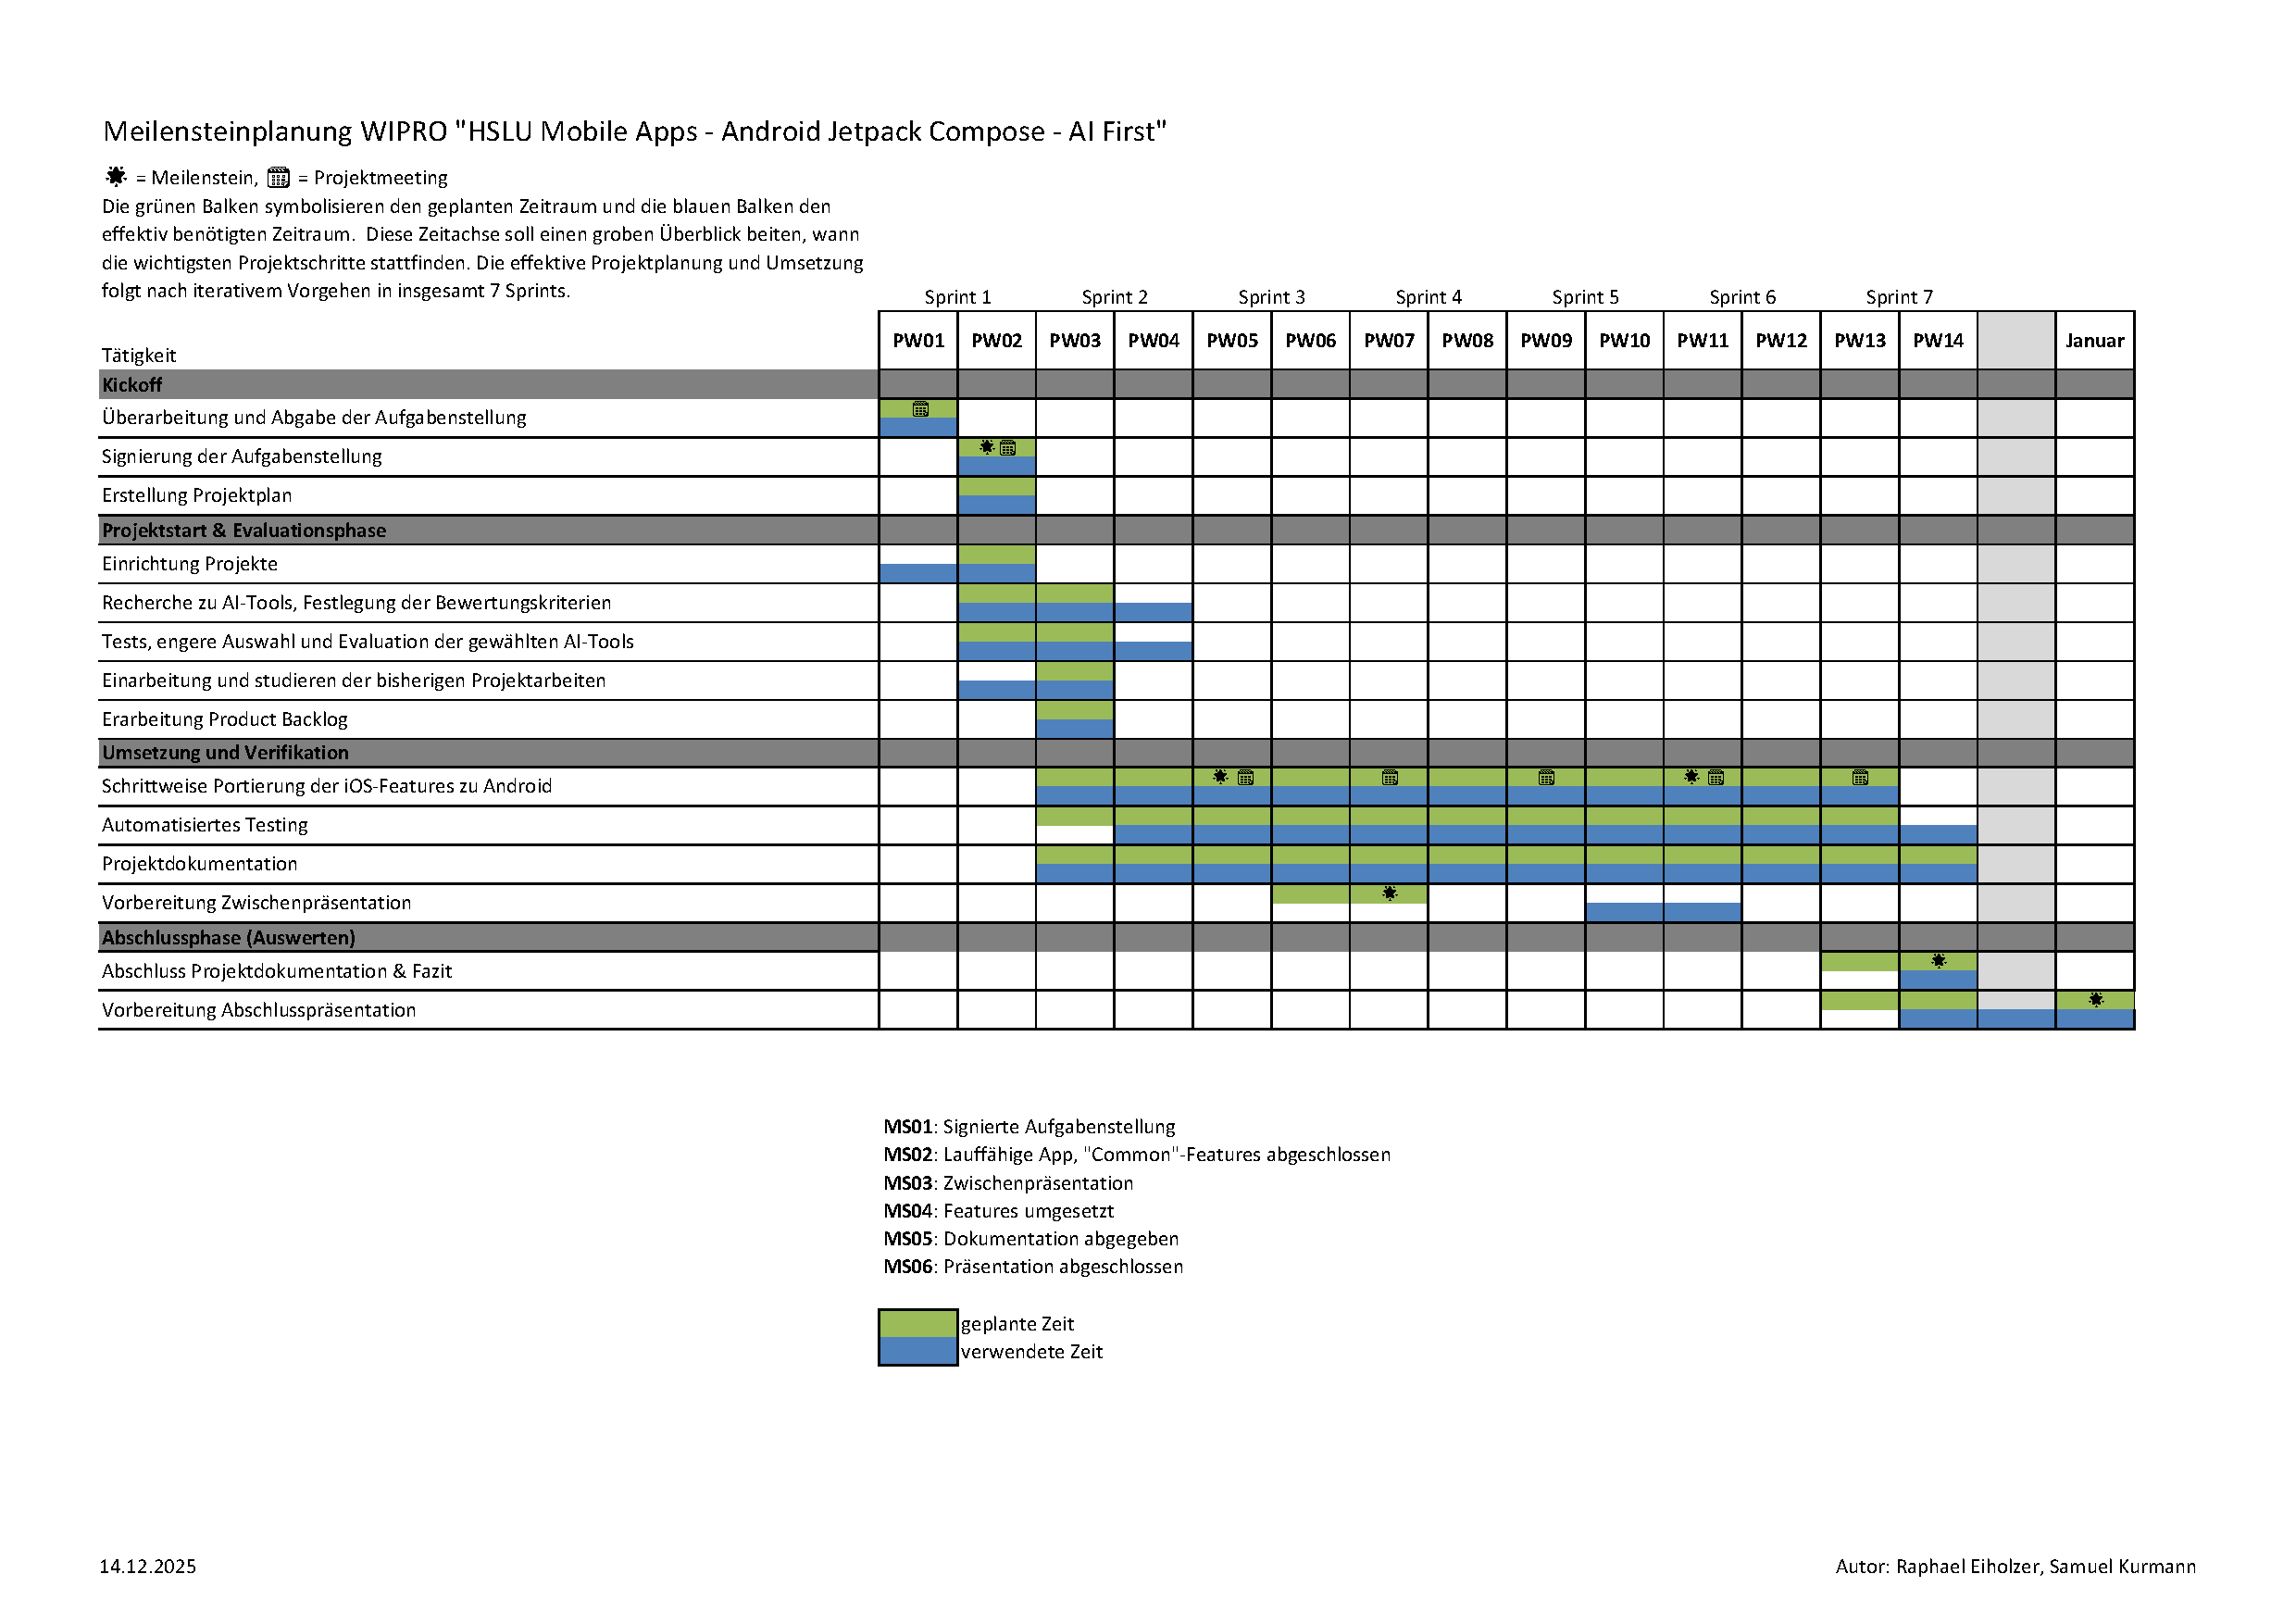
\includegraphics[width=0.85\textwidth]{Fotos/zeitplan.png}
    \caption{Meilensteinplan des Projekts}
    \label{fig:meilensteinplan}
\end{figure}\newpage

\subsection{Agiles Vorgehen}
Die Umsetzung des Projekts erfolgte nach einem agilen Vorgehen, angelehnt an
Scrum. Die Arbeit wurde in zweiwöchige Sprints unterteilt, woraus sich insgesamt
sieben Sprints ergaben. Vor jedem Sprint wurde im Team gemeinsam besprochen,
welche Aufgaben im kommenden Zeitraum umgesetzt werden sollen und wer welche
Arbeiten übernimmt.

\begin{figure}[H]
    \centering
    \includegraphics[width=0.35\textwidth]{Fotos/sprint_cycle.png}
    \caption{Darstellung des Scrum-Prozesses im Projekt} \parencite{atlassian_atlassian_nodate}
    \label{fig:scrum}
\end{figure}

Dieses Vorgehen ermöglichte ein effizientes Arbeiten, da Aufgaben flexibel
verteilt und bei freier Kapazität jederzeit neue Issues übernommen werden
konnten. Da alle Aufgaben und der aktuelle Projektstand in GitLab erfasst
waren, hatte auch der Auftraggeber jederzeit Einblick in den Fortschritt des
Projekts.

Zur Nachvollziehbarkeit des Projektverlaufs sind die Sprint-Backlogs als
grafische Übersicht im Anhang dokumentiert und zeigen den Fortschritt über die
gesamte Projektdauer hinweg (siehe ~\ref{anhang:sprintboard-1}).

\vspace{1.0em}
\begin{figure}[H]
    \centering
    \includegraphics[width=0.99\textwidth]{Fotos/sprintplanung-1.png}
    \caption{Backlogs in GitLab zu Projektbeginn}
    \label{fig:backlog}

\end{figure}\newpage

\subsubsection{Issues}
Alle Aufgaben im Projekt wurden als Issues in GitLab erfasst. Diese wurden
meist als einfache User Stories formuliert und mit einer kurzen
\textit{Definition of Done} (DoD) ergänzt. Dadurch war von Beginn an klar,
was zu einer Aufgabe gehört und wann sie als abgeschlossen gilt. Dies half, 
die Anforderungen besser zu verstehen und Missverständnisse zu
vermeiden.

Für jede Aufgabe wurde die aufgewendete Zeit direkt im jeweiligen Issue
dokumentiert. So konnte der Arbeitsaufwand über die gesamte Projektlaufzeit
hinweg nachvollzogen werden und es war jederzeit ersichtlich, wie viel Zeit
in welche Themen investiert wurde (siehe Anhang~\ref{anhang:zeit}).

\begin{figure}[H]
    \centering
    \includegraphics[width=0.7\textwidth]{Fotos/issue-userstory-dod.png}
    \caption{Beispiel einer User Story mit Definition of Done (DoD)}
    \label{fig:userstory}
\end{figure}

\subsection{Eingesetzte Programme/Tools}
Während der Projektdauer wurden diese Programme und Tools genutzt, um die Entwicklung, 
Dokumentation und die Organisation des Projekts zu unterstützen.

\vspace{0.6em}
\begin{table}[H]
\centering
\begin{tabular}{|l|p{12cm}|}
\hline
\textbf{Werkzeug} & \textbf{Einsatz im Projekt} \\
\hline
Git & Versionsverwaltung des Quellcodes \\
\hline
GitLab & Issue-Tracking, Sprint-Planung und Projektübersicht \\
\hline
OneNote & Persönliche Notizen, Skizzen und Screenshots während der Entwicklung \\
\hline
OneDrive & Zentrale Ablage für Projektdokumente und organisatorische Dateien \\
\hline
Latex & Erstellung und Formatierung der Projektdokumentation \\
\hline
VS Code & Editor zur Erstellung der Dokumentation \\
\hline
GitHub & Hosting des Dokumentations-Quellcodes \\
\hline
Android Studio & Endwicklungsumgebung für die Android-Applikation \\
\hline
Cursor & Endwicklungsumgebung mit AI-Features \\
\hline
Microsoft Teams & Kommunikation im Team und Meetings mit dem Auftraggeber \\
\hline
\end{tabular}
\caption{Eingesetzte Werkzeuge im Projekt}
\label{tab:werkzeuge}
\end{table}\clearpage


\subsection{Risikomanagement}
Zu Beginn des Projekts wurde eine Risikoanalyse erstellt, um die grössten Risiken frühzeitig zu identifizieren und entsprechende Gegenmassnahmen zu planen.  
Die Risiken wurden jeweils hinsichtlich Eintrittswahrscheinlichkeit und Auswirkung bewertet.  
Das Produkt dieser beiden Faktoren bestimmte den Gesamtrisiko-Wert und erlaubte es, die kritischsten Risiken zu priorisieren.  

Für jedes Risiko wurden präventive Massnahmen festgelegt, um die Eintrittswahrscheinlichkeit oder die Auswirkungen zu minimieren.  
Nach Umsetzung dieser Massnahmen wurde die Bewertung erneut vorgenommen, um verbleibende Risiken zu identifizieren und ihre Entwicklung über die Projektlaufzeit zu beobachten.  

\begin{figure}[H]
    \centering
    \includegraphics[width=0.4\textwidth]{Fotos/risikomatrix.png}
    \caption{Risikoanalyse und Risikomatrix des Projekts}
    \label{fig:risikomatrix}
\end{figure}

Die Risikoanalyse wurde während der gesamten Projektdauer regelmässig überprüft und aktualisiert.  
Am Ende jedes Sprints wurde die aktuelle Risikosituation besprochen und mögliche Massnahmen eingeleitet.  
Die drei grössten Risiken wurden zusätzlich an den Auftraggeber übermittelt, um Transparenz über den Projektfortschritt und potenzielle Herausforderungen sicherzustellen.
Die gesamte Risikoanalyse ist im Anhang zu finden (siehe Anhang~\ref{anhang:risk}).


\chapter{Realisierung}
Erläutere die Umsetzung, Architektur, Implementierungsdetails usw.
\input{LaTeX-Files/Network_Feature.tex}

\subsection{Fastlane}

Das Fastlane-Setup für die Android-App automatisiert den Build- und Deployment-Prozess für beide Tenants (HSLU I und HSLU TA). 
Anstatt separate Fastfiles pro Tenant zu verwenden wie das im Android-XML Projekt der Fall ist, wurde ein einheitliches, parametrisiertes Fastfile implementiert, 
das Redundanzen eliminiert und die Wartbarkeit verbessert. Das Fastfile unterstützt Debug- und Release-Builds sowie automatische Uploads zu Google Play Store in verschiedenen Tracks (Beta, Internal, Production).

\subsubsection*{Ziel und Motivation}

Das Hauptziel besteht darin, die CI/CD-Pipeline zu vereinfachen und Redundanzen zu eliminieren. 
Durch die Parametrisierung mit dem \texttt{tenant}-Parameter kann ein einziges Fastfile für beide Tenants verwendet werden, 
was die Wartbarkeit erheblich verbessert. Zusätzlich werden alle sensiblen Daten (Keystores, API-Keys) sicher in einem separaten Git-Repository gespeichert und verschlüsselt, 
sodass sie nicht im Haupt-Repository liegen.

Ein weiteres wichtiges Ziel ist die Automatisierung des gesamten Build- und Deployment-Prozesses, 
von der Kompilierung über die Signierung bis hin zum Upload in den Google Play Store. 
Dies reduziert manuelle Fehler und beschleunigt den Release-Prozess erheblich.

\subsubsection*{Umsetzung / Funktionsweise}

Die Implementierung basiert auf einem zentralen \texttt{before\_all}-Block, der die Initialisierung und Konfiguration für alle Lanes übernimmt. 
Das Fastfile verwendet Dotenv für die Verwaltung von Secrets und parametrisiert alle tenant-spezifischen Werte. 
Der \texttt{before\_all}-Block wird vor jeder Lane ausgeführt und übernimmt die Validierung des \texttt{tenant}-Parameters, 
die Definition von Pfaden sowie das Mapping von Tenant-Namen zu Android-Modulen und Package-IDs.

Die tenant-spezifischen Umgebungsvariablen (Keystore-Passwörter, API-Keys, etc.) werden aus \texttt{.env.secret} geladen 
und in generische Variablen gemappt, sodass alle Lanes die gleichen Variablennamen verwenden können.

\paragraph*{Lanes}

Das Fastfile definiert vier Haupt-Lanes, die in der folgenden Tabelle beschrieben sind:

\begin{table}[h]
\centering
\begin{tabularx}{\textwidth}{|l|X|}
\hline
\textbf{Lane} & \textbf{Beschreibung} \\
\hline
\texttt{build\_debug} & Erstellt einen Debug-Build ohne Signierung. Führt \texttt{gradle clean assemble} für das entsprechende Tenant-Modul aus und kopiert die Artefakte in den Output-Ordner. Wird hauptsächlich für lokale Tests verwendet. \\
\hline
\texttt{build\_release} & Erstellt einen signierten Release-Build. Lädt den verschlüsselten Keystore aus dem Zertifikats-Repository, entschlüsselt ihn, erstellt die \texttt{keystore.properties}-Datei für Gradle und führt \texttt{gradle clean bundle} aus. Das signierte AAB wird in den Output-Ordner kopiert. \\
\hline
\texttt{beta} & Baut ein signiertes Release-Bundle und lädt es in den Google Play Store hoch. Standardmässig wird der Beta-Track verwendet, kann aber über den \texttt{track:}-Parameter überschrieben werden (z.\,B. \texttt{track:internal}). Lädt sowohl Keystore als auch Google Play API-Key aus dem Zertifikats-Repository. Ruft intern \texttt{build\_release} auf und lädt anschliessend das AAB hoch. \\
\hline
\texttt{release} & Analog zu \texttt{beta}, lädt jedoch explizit in den Production-Track des Google Play Stores. Wird für finale Releases verwendet. \\
\hline
\end{tabularx}
\caption{Übersicht der Fastlane-Lanes}
\label{tab:fastlane-lanes}
\end{table}

\paragraph*{Hilfsfunktionen}

Das Fastfile verwendet mehrere Hilfsfunktionen zur Verwaltung von Zertifikaten und Konfiguration:

\begin{itemize}
    \item \texttt{download\_from\_certs\_repo}: Klont das Zertifikats-Repository und entschlüsselt eine Datei (typischerweise den Keystore) mit OpenSSL (AES-256-CBC).
    \item \texttt{download\_from\_certs\_repo\_full}: Erweiterte Variante, die sowohl Keystore als auch Google Play API-Key entschlüsselt.
    \item \texttt{create\_keystore\_properties}: Erstellt die \texttt{keystore.properties}-Datei dynamisch, die von Gradle für die Signierung verwendet wird.
    \item \texttt{clean\_directory}: Entfernt temporäre Zertifikatsdateien nach dem Build, um Sicherheitsrisiken zu minimieren.
\end{itemize}

\subsubsection*{Verwendung und Sicherheit}

Die Verwendung erfolgt durch Aufruf von Fastlane mit dem \texttt{tenant}-Parameter: 
\texttt{fastlane <lane> tenant:hslui} oder \texttt{fastlane <lane> tenant:hsluta}. 
Ohne diesen Parameter bricht Fastlane mit einer Fehlermeldung ab.

Alle sensiblen Daten (Keystores, API-Keys) werden in einem separaten Git-Repository gespeichert und mit OpenSSL verschlüsselt (AES-256-CBC). 
Die Passwörter für die Entschlüsselung werden aus \texttt{.env.secret} geladen, das nicht im Repository gespeichert wird, 
sondern von der CI/CD-Pipeline zur Laufzeit erstellt wird. Die Keystore-Properties-Datei wird dynamisch erstellt 
und nach dem Build gelöscht, um Sicherheitsrisiken zu minimieren.

Die Upload-Funktionalität unterstützt verschiedene Tracks im Google Play Store. 
Der Standard-Track für \texttt{beta} ist "beta", kann aber über den \texttt{track:}-Parameter überschrieben werden (z.\,B. \texttt{track:internal}). 
Changelogs werden bewusst übersprungen, da diese manuell im Google Play Console verwaltet werden.

Das Fastfile ist erweiterbar für weitere Tenants, indem einfach ein neuer \texttt{when}-Fall im 
\texttt{before\_all}-Block hinzugefügt wird und die entsprechenden Umgebungsvariablen in \texttt{.env.secret} definiert werden.


\chapter{Validierung und Evaluation}
Beschreibe, wie die Lösung überprüft, getestet oder bewertet wurde.

\section{Teststrategie – Android Multi-Tenant App (Jetpack Compose)}

Todo Raphi: Überarbeitung

\subsection{Ausgangslage}
In der bisherigen mobilen Applikationslandschaft – sowohl bei der iOS-App als auch bei der älteren Android-App auf XML-Basis – war die Testabdeckung sehr gering.  
Es existierten nur wenige automatisierte Tests, meist oberflächliche oder technische Tests ohne echten Bezug zur Geschäftslogik. Dadurch war die Qualitätssicherung stark manuell geprägt, und Änderungen am Code konnten nur mit hohem Aufwand überprüft werden.

Mit der Neuentwicklung der Android-App auf Basis von Jetpack Compose soll dieser Zustand deutlich verbessert werden. Ziel ist es, eine strukturierte, modulare und wartbare Teststrategie aufzubauen, die langfristig eine hohe Codequalität und Stabilität sicherstellt.

\subsection{Zielsetzung}
\begin{itemize}
    \item Aufbau einer einheitlichen Testarchitektur über alle Module hinweg
    \item Erhöhung der Testabdeckung, insbesondere in der Business Logic und bei den ViewModels
    \item Klare Trennung zwischen Unit-, Integrations- und UI-Tests
    \item Einführung moderner Testframeworks mit JUnit 5 (Jupiter)
\end{itemize}

\subsection{Umsetzung}

\subsubsection{Testarten und Vorgehen}

\paragraph{Unit Tests (\texttt{src/test/})}
Ziel: Isolierte Tests einzelner Klassen und Methoden ohne Android-Abhängigkeiten

Frameworks: JUnit 5, Mockito oder MockK

Fokus: Business Logic, Datenmodelle und ViewModels

Vorgehen:
\begin{itemize}
    \item Jede logische Komponente (z.\,B. Parser, Berechnungen, ViewModels) erhält eigene Unit Tests
    \item Abhängigkeiten werden gemockt, um reine Logiktests zu ermöglichen
    \item Tests folgen dem AAA-Prinzip (Arrange – Act – Assert) und klaren Namenskonventionen
\end{itemize}

\noindent Beispiel:
\begin{lstlisting}
@Test
fun `should return correct sum when valid input provided`() {
    val calculator = Calculator()
    val a = 5
    val b = 3
    val result = calculator.add(a, b)
    assertEquals(8, result)
}
\end{lstlisting}

\paragraph{Integration- und UI-Tests (\texttt{src/androidTest/})}
Ziel: Überprüfung des Zusammenspiels mehrerer Komponenten im echten Android-Kontext

Frameworks: JUnit 5, Espresso, Jetpack Compose Testing

Fokus: UI-Verhalten, Datenfluss, Netzwerk- und Datenbankinteraktionen

Vorgehen:
\begin{itemize}
    \item Tests laufen mit Android Emulator oder Gerät
    \item Überprüfen reale Benutzerinteraktionen (z.\,B. Klicks, Eingaben, Navigationsflüsse)
    \item Fokus auf Haupt-Userflows und kritische Systempfade
\end{itemize}

\subsection{Struktur und Modularität}
Jedes Modul (z.\,B. App, Common, Features) verfügt über eigene Testverzeichnisse:
\begin{itemize}
    \item \texttt{src/test/} → Unit Tests  
    \item \texttt{src/androidTest/} → Instrumentierte Integration- und UI-Tests  
\end{itemize}

Diese klare Trennung ermöglicht modulunabhängiges Testen, parallele Ausführung und einfache Erweiterung der Testbasis.

\subsection{Zielwerte und Qualität}
\begin{itemize}
    \item Unit-Test-Abdeckung: mindestens 80\,\%
    \item Integration/UI-Tests: Fokus auf kritische Anwendungsfälle
    \item CI/CD-Integration: Automatische Testausführung bei jedem Build
    \item Langfristig: Schrittweise Ausweitung auf alle bestehenden Module
\end{itemize}

\subsection{Fazit}
Mit der neuen Jetpack-Compose-Architektur wurde eine klare und moderne Teststruktur geschaffen, die auf JUnit 5 basiert und sowohl Unit- als auch Android-Tests konsequent trennt.  
Damit wird erstmals eine nachhaltige Testbasis gelegt, um Qualität, Stabilität und Wartbarkeit der App langfristig sicherzustellen.


Im Projektauftrag der WIPRO ist festgelegt, dass die Android-Applikation nach
einem \emph{AI-First}-Ansatz entwickelt werden soll. Ziel ist es dabei, künstliche
Intelligenz bewusst und aktiv in den Entwicklungsprozess einzubinden und deren
Nutzen im realen Projektalltag zu prüfen.

Damit dieser Ansatz sinnvoll umgesetzt werden kann, ist eine Auswahl
geeigneter AI-Tools notwendig. Da eine Vielzahl unterschiedlicher KI-Lösungen
existiert und nicht für jedes Tool ein kostenpflichtiges Abonnement abgeschlossen
werden kann, wurde zu Beginn eine kleine Evaluation durchgeführt. Ziel dieser
Evaluation ist es, jene Tools zu identifizieren, die im Kontext der Android-
Entwicklung den grössten praktischen Mehrwert bieten.

Die Evaluation basiert auf einer Kombination aus vorhandenen
Erkenntnissen sowie praktischen Erfahrungen aus Selbstexperimenten mit den
kostenlosen Versionen der jeweiligen Tools. Nach Abschluss dieser Analyse wurde
eine fundierte Entscheidung für ein primäres Tool getroffen, welches im weiteren
Projektverlauf auch in der kostenpflichtigen Version eingesetzt wird, um den
AI-First-Ansatz konsequent und effektiv umzusetzen.

\subsection{Vorarbeiten}

Im Vorfeld dieses Wirtschaftsprojekts wurde im Rahmen des Moduls
\emph{Wissenschaftliches Schreiben \& Forschungsmethodik (WSFM)} im
September 2025 bereits untersucht, wie der Einsatz von AI-Tools im
Kontext der Softwareentwicklung sinnvoll und methodisch korrekt
evaluiert werden kann. Ziel dieser Vorarbeit war es, zu klären, mit
welchen Ansätzen sich der Nutzen von AI-Tools messen lässt und wie eine
mögliche Zeitersparnis wissenschaftlich belegt werden könnte
(siehe Anhang~\ref{anhang:wsfm}).

Das Ergebnis dieser Vorarbeit war die Erkenntnis, dass ein
streng wissenschaftlicher Ansatz mit Umfragen, kontrollierten
Experimenten, Tests mit erfahrenen Entwicklerinnen sowie Interviews
einen sehr hohen organisatorischen und zeitlichen Aufwand erfordern
würde. Für den Rahmen dieses Wirtschaftsprojekts hätte ein solches
Vorgehen den Umfang deutlich überschritten und wäre nicht realistisch
umsetzbar gewesen.

Diese Einschätzung wurde auch im Austausch mit dem Auftraggeber
diskutiert und gemeinsam im Projektstatus-Meeting vom 25.09.2025
bestätigt (siehe Anhang~\ref{anhang:meeting25092025}). Aus diesem Grund
wurde bewusst auf eine vollständig wissenschaftliche Evaluation
verzichtet.

Stattdessen wurde ein pragmatischer, praxisnaher Ansatz gewählt. Die
Evaluation der AI-Tools erfolgte direkt anhand des konkreten
Projektkontexts, insbesondere durch die Übertragung grösserer
Codebestandteile von Swift nach Kotlin. Dieselben Aufgabenstellungen
wurden mehreren AI-Tools vorgelegt und die Resultate schrittweise
beurteilt. Dabei standen für uns Kriterien wie Verständlichkeit,
Korrektheit, Anpassungsaufwand und tatsächlicher Nutzen im
Projektalltag im Vordergrund. Auf dieser Basis konnte ein fundiertes
Fazit gezogen werden, welche Tools sich für unseren Anwendungsfall am
besten eignen (vgl. ebenfalls Anhang~\ref{anhang:meeting25092025}).

\subsection{Aufgabenstellung für die AI Tools}
Wir haben mehreren AI-Tools, die wir entweder bereits selbst genutzt haben,
von denen wir viel Positives gehört haben oder die in wissenschaftlichen
Untersuchungen häufig genannt werden, dieselbe Aufgabenstellung vorgelegt.
Ziel war es, die jeweiligen Antworten zu analysieren und miteinander zu
vergleichen, um einen ersten Eindruck zu erhalten, welches Tool die
umfangreichste und für unseren Anwendungsfall sinnvollste Analyse liefert.

Die vollständige und detaillierte Aufgabenstellung ist im Anhang dokumentiert
(siehe Anhang~\ref{aufgabenstellung-ai-tools}).

\subsection{Analyse der evaluierten AI-Tools}
Im Rahmen der Evaluation wurden die AI-Tools ChatGPT, Grok (xAI), DeepSeek und
Cursor betrachtet. Allen Tools wurde dieselbe Aufgabenstellung vorgegeben, um
ihre Fähigkeiten zur Analyse sowie zur Unterstützung bei der
Android-App-Entwicklung vergleichbar beurteilen zu können.

ChatGPT lieferte eine fundierte Antwort mit ausreichender Tiefe für eine erste
technische Einschätzung. Besonders hilfreich war das breite
Cross-Plattform-Wissen in den Bereichen iOS und Android sowie der Vergleich
zwischen SwiftUI und Jetpack Compose. Zudem wurden sinnvolle Hinweise zu
Architektur und Testing gegeben. Die Pro-Version von ChatGPT kostet 23 Euro pro
Monat. Die vollständige Antwort ist im Anhang dokumentiert
(siehe Anhang~\ref{antwort-chatgpt}).

Auch Grok von xAI erzeugte eine strukturierte und nachvollziehbare Antwort, die
einen guten Überblick über mögliche Lösungsansätze bietet. Dabei wurden
verschiedene technische Optionen aufgezeigt und priorisiert. Mit dem Modell
„grok-code-fast-1“ richtet sich Grok gezielt an Entwickleraufgaben mit Fokus auf
Effizienz und Code-Qualität. Die SuperGrok-Version kostet 30 Euro pro Monat. Die
vollständige Antwort ist im Anhang zu finden
(siehe Anhang~\ref{antwort-grok}).

DeepSeek überzeugte insbesondere durch die detaillierte Auswertung der
Aufgabenstellung sowie der bereitgestellten Screenshots und Codeausschnitte.
Die Antworten enthielten konkrete Entwürfe für die Android-App, ergänzende
Strategien sowie erste Codebeispiele. Zusätzlich wurde eine strukturierte
Checkliste der notwendigen Umsetzungsschritte bereitgestellt. DeepSeek ist
kostenlos nutzbar und bietet keine kostenpflichtigen Abonnements an. Die
vollständige Antwort ist im Anhang dokumentiert
(siehe Anhang~\ref{antwort-deepseek}).

Cursor unterscheidet sich von den anderen Tools dadurch, dass es sich nicht um
eine reine Web-KI handelt, sondern um eine eigenständige Anwendung mit IDE-nahem
Frontend. Ganze Projektstrukturen können geöffnet und analysiert werden, wodurch
der KI jederzeit der vollständige Projektkontext zur Verfügung steht. Cursor
selbst ist kein eigenes Sprachmodell, sondern dient als Oberfläche zur Nutzung
verschiedener LLMs. Dieser Ansatz bietet einen klaren Vorteil gegenüber
klassischen Web-Tools, da Zusammenhänge im Projekt besser erkannt werden können.
Die Pro-Version von Cursor kostet 20 Euro pro Monat. Die vollständige Antwort ist
im Anhang dokumentiert (siehe Anhang~\ref{antwort-cursor}).

\subsection{Vergleich}

\begin{table}[H]
  \centering
  \small
  \setlength{\tabcolsep}{6pt}
  \renewcommand{\arraystretch}{1.2}
  \begin{tabularx}{\textwidth}{l>{\raggedright\arraybackslash}X>{\raggedright\arraybackslash}X>{\raggedright\arraybackslash}X}
    \toprule
    \textbf{KI} &
    \textbf{Stärken / beobachtete Fähigkeiten} &
    \textbf{Schwächen / Unsicherheiten} &
    \textbf{Eignung} \\
    \midrule
    Grok (xAI) &
    xAI hat mit „grok-code-fast-1“ ein Modell für Entwickler-Aufgaben (Agentic Coding) vorgestellt; Effizienz/Qualität im Fokus; funktioniert auch als Backend in Tools wie Cursor. &
    Relativ jung; unklare Reife/Plattformtiefe; unklar, wie gut Apple/Android-SDKs abgedeckt sind. &
    Spannend mit aktueller Grok-Version; mit guter Prompt-Strategie evtl. starker Konkurrent zu Claude. \\
    \addlinespace
    DeepSeek &
    Kostengünstige, vergleichbare Alternative; Integration in IDE-Umgebungen möglich. &
    Weniger öffentlich dokumentierte Benchmarks; evtl. unreifer bei Edge-Cases / Plattformcode. &
    Gute Ergänzung, v. a. wenn Kosten zählen; für kritische Teile menschliches Review einplanen. \\
    \addlinespace
    ChatGPT &
    Sehr stark bei Cross-Plattform-Wissen (iOS/Android, SwiftUI/Compose, Flutter, RN); bewährt; gute Architektur- und Testing-Hinweise. &
    Token-Limits bei sehr grossen Codebasen (ausser Enterprise/Pro); potenzielle Halluzinationen → Review nötig. &
    Top-Option neben Claude; stark für Architektur/Best Practices. \\
    \addlinespace
    Cursor &
    IDE-Frontend, das verschiedene Modelle einbindet; verbessert Workflow und Kontext im Editor. &
    Keine eigene KI; Leistung hängt vom gewählten Modell ab. &
    Als Interface/Workflow-Booster zusammen mit starkem Modell nutzen (z. B. Grok/ChatGPT/Claude). \\
    \bottomrule
  \end{tabularx}
  \caption{Auswertung der KI in Tabellenform}
\end{table}

\subsection{Auswertung anhand von Bewertungskriterien}

Um die evaluierten AI-Tools nicht nur qualitativ zu vergleichen, sondern auch
eine nachvollziehbare Entscheidungsgrundlage zu schaffen, wurden klare
Bewertungskriterien definiert. Diese Kriterien orientieren sich direkt am
Projektalltag und daran, welchen tatsächlichen Mehrwert ein Tool während der
Entwicklung bietet.

Die Bewertung erfolgte subjektiv auf Basis unserer praktischen Erfahrungen im
Projekt. Jedes Kriterium wurde auf einer Skala von 1 (sehr schlecht) bis 5
(sehr gut) beurteilt.

Die folgenden Kriterien wurden für die Auswertung herangezogen:
\begin{itemize}
    \item \textbf{Code-Qualität}: Struktur, Lesbarkeit und Nähe zu Clean-Code-Prinzipien
    \item \textbf{Korrektheit und Funktionsfähigkeit}: fachlich korrekte und lauffähige Resultate
    \item \textbf{Anpassungsaufwand}: benötigte Nacharbeit bis zur produktiven Nutzung
    \item \textbf{Verständnis des Kontexts}: Fähigkeit, Projektstruktur und Zusammenhänge zu erfassen
    \item \textbf{Zeitersparnis im Projektalltag}: tatsächlicher Effizienzgewinn gegenüber manueller Umsetzung
\end{itemize}

\begin{table}[H]
    \centering
    \small
    \setlength{\tabcolsep}{6pt}
    \renewcommand{\arraystretch}{1.2}
    \begin{tabularx}{\textwidth}{lccccc}
        \toprule
        \textbf{KI-Tool} &
        \textbf{Code-Qualität} &
        \textbf{Korrektheit} &
        \textbf{Anpassungs\-aufwand} &
        \textbf{Kontext\-verständnis} &
        \textbf{Zeitersparnis} \\
        \midrule
        ChatGPT & 4 & 4 & 3 & 3 & 4 \\
        Grok (xAI) & 4 & 3 & 3 & 3 & 3 \\
        DeepSeek & 3 & 3 & 2 & 2 & 3 \\
        Cursor & \textbf{5} & \textbf{5} & \textbf{4} & \textbf{5} & \textbf{5} \\
        \bottomrule
    \end{tabularx}
    \caption{Bewertung der AI-Tools anhand definierter Kriterien (1 = schlecht, 5 = sehr gut)}
    \label{tab:ai-bewertung}
\end{table}

\subsubsection*{Fazit der Auswertung}

Auf Basis der definierten Kriterien und der praktischen Nutzung im Projekt
konnte Cursor als klarer Gewinner identifiziert werden. Ausschlaggebend war
insbesondere das sehr gute Kontextverständnis durch den Zugriff auf die gesamte
Projektstruktur sowie der daraus resultierende deutliche Zeitgewinn im
Projektalltag.

Während sich die zugrunde liegenden Sprachmodelle in ihrer grundsätzlichen
Qualität nur begrenzt unterscheiden, bietet Cursor durch sein IDE-nahes
Frontend einen entscheidenden Mehrwert. Für unser Projekt erwies sich diese
Kombination aus starkem Modell und vollständigem Projektkontext als die
effektivste Lösung für einen konsequenten AI-First-Ansatz.

\subsection{Detaillierter Fragen zu Cursor}
Da wir von Cursor sehr überzeugt sind, insbesondere weil es sich um eine
Applikation mit eigenem Frontend handelt, können ganze Ordnerstrukturen
geöffnet und analysiert werden, ähnlich wie in Visual Studio Code. Dadurch
erhält die KI einen direkten Überblick über die gesamte Codebasis. Dies
erleichtert es deutlich, präzisere und sinnvollere Antworten zu erhalten, da
der Kontext einzelner Codestellen für die KI jederzeit klar ist. Im Gegensatz
zu klassischen webbasierten Tools, bei denen nur selektiv hochgeladener Code
betrachtet wird, entstehen so weniger Fehlinterpretationen.

Nachfolgend ist ein Screenshot dargestellt, der exemplarisch zeigt, wie gut
eine einzelne Datei analysiert werden kann, wenn der vollständige
Projektkontext vorhanden ist. In diesem Beispiel wurde die KI gefragt, welche
Aufgabe die Datei \texttt{CommonApplicationBaseModuleLoader.swift} übernimmt
und wie sie im Zusammenhang mit dem restlichen Projekt steht. Dabei wird
deutlich, dass Cursor die Projektstruktur ganzheitlich analysiert und
relevante Codestellen gezielt hervorhebt, was das Verständnis komplexer
Zusammenhänge erheblich erleichtert.

\begin{figure}[H]
  \centering
  \includegraphics[width=0.6\textwidth]{Fotos/Cursor_1.png}
  \caption{Analysebeispiel in Cursor}
  \label{fig:cursor-example}
\end{figure}


\subsection{Fazit}

Auf Basis der durchgeführten Evaluation und der praktischen Erfahrungen im
Projekt sind wir zum Schluss gekommen, dass Cursor in Kombination mit einem
der evaluierten Sprachmodelle für unseren Anwendungsfall die beste Lösung
darstellt. Ausschlaggebend war insbesondere der Zugriff auf den vollständigen
Projektkontext, der es der KI ermöglicht, deutlich sinnvolleren und besser
integrierten Code zu erzeugen als klassische webbasierten Tools.

Die zugrunde liegenden Large Language Models unterscheiden sich aus unserer
Sicht im Kern weniger stark voneinander, als es auf den ersten Blick scheint.
Der entscheidende Mehrwert entsteht vielmehr durch das Umfeld, in dem das
Modell eingesetzt wird. Hier bietet Cursor durch sein IDE-nahes Frontend klare
Vorteile im Projektalltag.

Der Cursor Pro Plan erweist sich dabei grundsätzlich als ausreichend, da im
Auto-Modus für kleinere Anfragen kostengünstige oder kostenfreie APIs genutzt
werden und kostenpflichtige Modelle nur bei umfangreicheren Abfragen zum
Einsatz kommen. Dennoch ist zu beachten, dass bei intensiver Nutzung oder bei
mehreren gleichzeitig arbeitenden Personen zusätzliche Kosten entstehen
können.

Im weiteren Projektverlauf wurde zudem Rücksprache mit dem Dozenten gehalten,
welche AI-Tools seitens der Hochschule Luzern bevorzugt werden. Dabei zeigte
sich, dass ChatGPT offiziell unterstützt wird. Um diese Vorgabe einzuhalten
und gleichzeitig nicht auf die Vorteile von Cursor verzichten zu müssen,
wurde Cursor so konfiguriert, dass ausschliesslich die ChatGPT-API verwendet
wird. Dadurch konnte ein sinnvoller Kompromiss gefunden werden, der sowohl
den institutionellen Rahmenbedingungen als auch den praktischen Anforderungen
des Projekts gerecht wird.

\subsection{Erfahrungen mit dem AI-First-Ansatz}

Während der gesamten Projektlaufzeit wurde der \emph{AI-First}-Ansatz
konsequent verfolgt und Cursor aktiv in den Entwicklungsprozess integriert.
Dabei konnten sowohl positive Effekte als auch klare Grenzen des Einsatzes
von KI beobachtet werden. Insgesamt hat sich gezeigt, dass AI den
Entwicklungsprozess deutlich unterstützen und beschleunigen kann, jedoch
weiterhin eine kritische Bewertung und fachliche Kontrolle durch die
Entwickler notwendig bleibt.

Eine detaillierte Reflexion der gemachten Erfahrungen, insbesondere zu
Stärken, Schwächen und Grenzen von AI-gestützter Entwicklung, erfolgt im
Kapitel zur Reflexion (siehe Abschnitt~\ref{sec:ai-reflexion}).


\chapter{Ausblick}
Welche zukünftigen Arbeiten, Verbesserungen oder Erweiterungen sind denkbar?

% ================== Anhänge ====================================================

\appendix
\chapter{Anhänge}
\section{Zusatzmaterial}
Screenshots, Diagramme, Code-Ausschnitte etc.

% ================== Verzeichnisse =============================================

\chapter*{Abkürzungs-, Abbildungs-, Tabellen-, KI-, Formelverzeichnis}
\addcontentsline{toc}{chapter}{Abkürzungs-, Abbildungs-, Tabellen-, KI-, Formelverzeichnis}

\section*{Abkürzungsverzeichnis}

\section*{Abbildungsverzeichnis}
\vspace{-4.5em}
\begingroup
\renewcommand{\listfigurename}{}
\let\clearpage\relax
\let\cleardoublepage\relax
\listoffigures
\endgroup

\section*{Tabellenverzeichnis}
\section*{KI-Verzeichnis}
\section*{Formelverzeichnis}

\chapter*{Literaturverzeichnis}
\printbibliography

% ================== Ende =======================================================

\end{document}